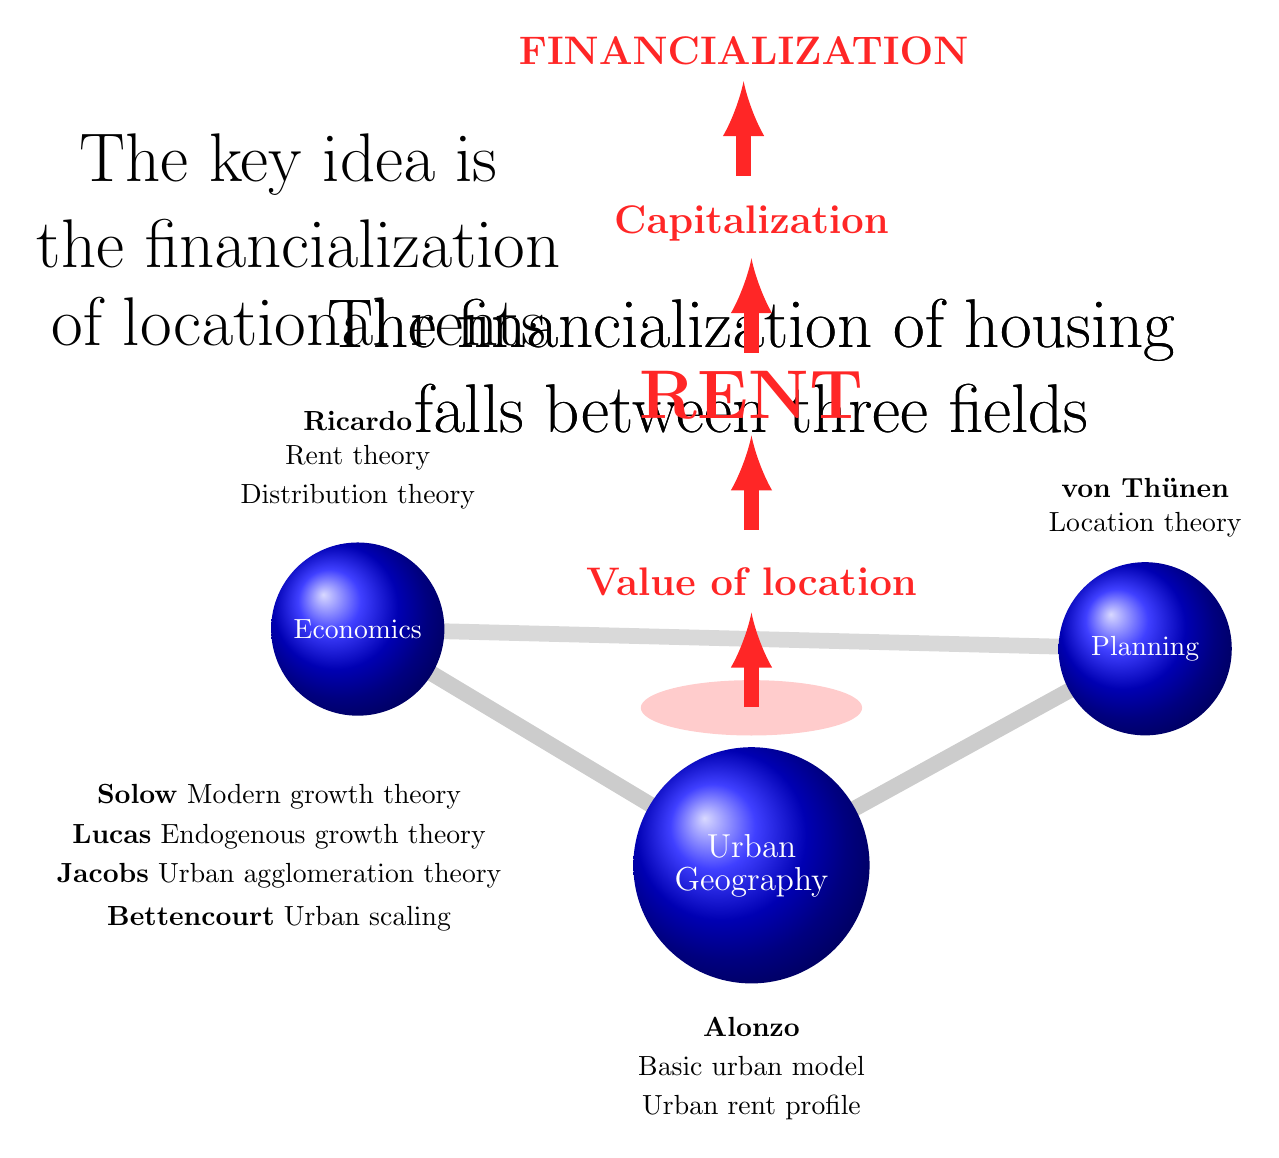
\begin{tikzpicture}{scale=.5}
% Find color for ball. Stop line short of node
\coordinate (planning) at (5,.75); % Preface
\coordinate (economics) at (-5,1); 
\coordinate (Ricardo) at (-5,1.4);
\coordinate (Solow) at (-6,1.25);
\coordinate (geography) at (0,-2); % History
\coordinate (finance) at (0,5); 

\draw [line width=2mm, black!15, ] (planning)--(economics);
\draw [line width=2mm, black!20, ] (geography)--(economics);
\draw [line width=2mm, black!20, ] (geography)--(planning);
%\draw [line width=2mm, black!25, ] (geography)--(finance);
%\draw [line width=2mm, black!20, ] (planning)--(finance);
%\draw [line width=2mm, black!20, ] (finance)--(economics);
%color=black!60!red
%\shade [ball color=blue!70] (5,5) circle (1.1cm)node[white] {\textbf{Planning}};
 
\node [circle,shading=ball,  minimum width=2.2cm, white, align=center] (ball) at (planning) {Planning};
\node [circle, shading=ball, minimum width=2.2cm, white, align=center] (ball) at (economics) {Economics};
\node [circle,shading=ball, minimum width=3cm, white, align=center] (ball) at (geography)[text width=2cm] {\large Urban \\ Geography};
%\node [circle, shading=ball, minimum width=2.4cm, white, align=center] (ball) at (finance)[text width=2cm] {Finance};
%\node at (-.3,-.1) [red] {\Large \textbf{RENT}};

\fill[red!20] (0,0) ellipse (40pt and 10pt);

\onslide<1>
{\node at (0, 4.8)[align=center, font=\Huge ]{The financialization of housing};
\node at (0, 3.8)[align=center, font=\Huge]  {falls between three fields};
};

\onslide<2>
{\node at (0, 4.8)[align=center, font=\Huge ]{The financialization of housing};
\node at (0, 3.8)[align=center, font=\Huge]  {falls between three fields};
};
% \onslide<2>{\node at (0, 5.8)[align=center]{\Huge I draw on  theories };
% \node at (0, 4.8)[align=center]{\Huge from multiple fields};
% };

\onslide<3>
{\node at (-5.75, 6.9)[align=center]{\Huge The key idea is };
\node at (-5.75, 5.9)[align=center]{\Huge the financialization};
\node at (-5.75, 4.9)[align=center]{\Huge  of locational rents};
};

\pause


\node at (planning) [above=1.8cm] {\textbf{von Th\"unen}};
\node at (planning) [above=1.3cm] {Location theory};

\node at (Ricardo) [above=2cm,]   {\textbf{Ricardo}};
\node at (Ricardo) [above=1.5cm] {Rent theory};
\node at (Ricardo) [above=1.0cm] {Distribution theory};

% \node at (Solow) [below=1.6cm, align=left] {\textbf{Solow:}};
\node at (Solow) [below=2.1cm, align=left] {\textbf{Solow} Modern growth theory};
\node at (Solow) [below=2.6cm, align=left] {\textbf{Lucas} Endogenous growth theory};
\node at (Solow) [below=3.1cm, align=left] {\textbf{Jacobs} Urban agglomeration theory};
\node at (Solow) [below=3.65cm, align=left] {\textbf{Bettencourt} Urban scaling};

\node at (geography) [below=1.8cm] {\textbf{Alonzo}};
\node at (geography) [below=2.3cm] {Basic urban model};
\node at (geography) [below=2.8cm] {Urban rent profile};
%\node [circle, shading=ball, minimum width=2.4cm, white, align=center] (ball) at (finance)[text width=2cm] {Finance};


\pause

%\node[red]at (1.2,0) {\large SPACE};
\begin{scope}[shift={(0,-.34)}]
\draw [line width=2mm, red!85, -latex ] (-.1, 7.1)--++(0,1.2)node[above=-.1] {\Large \textbf{FINANCIALIZATION}};
\draw [line width=2mm, red!85, -latex ] (0, 4.85)--++(0,1.2)node[above=-.1] {\Large \textbf{Capitalization}};
\draw [line width=2mm, red!85, -latex ] (0, 2.6)--++(0,1.2)node[above=-.1] {\Huge \textbf{RENT}};
\draw [line width=2mm, red!85, -latex ] (0, .35)--++(0,1.2)node[above] {\Large \textbf{Value of location}};
%\draw [line width=2mm, red!85, -latex ] (0, -2)--++(0,-.8)node[above=-.1]  {\Large \textbf{SPACE}};
\end{scope}
\end{tikzpicture}


% % JUST THE BOTTOM 3 BALLS FOR PLANNING, ECONOMICS AND URBAN GEOGRAPHY
% \begin{figure}
% \begin{tikzpicture}{scale=.5}
% % find color cotrol for ball. Tind way to stop line short of node
% \coordinate (planning) at (-5,1);%PREFACE
% \coordinate (economics) at (5,.75);%
%  \coordinate (geography) at (-.5,-2); %history
% \coordinate (finance) at (0,5); %

% \draw [line width=2mm, black!15, ] (planning)--(economics);
% \draw [line width=2mm, black!20, ] (geography)--(economics);
% \draw [line width=2mm, black!20, ] (geography)--(planning);

% %\draw [line width=2mm, black!25, ] (geography)--(finance);
% %\draw [line width=2mm, black!20, ] (planning)--(finance);
% %\draw [line width=2mm, black!20, ] (finance)--(economics);
% \node [circle,shading=ball, minimum width=2.1   cm, white, align=center] (ball) at (planning) {Planning};
% \node [circle,shading=ball, minimum width=2.2cm, white, align=center] (ball) at (economics) {Economics};
% \node [circle,shading=ball, minimum width=3cm, white, align=center] (ball) at (geography)[text width=2cm] {\large Urban\\ Geography};
% %\node [circle, shading=ball, minimum width=2.4cm, white, align=center] (ball) at (finance)[text width=2cm] {Finance};

% \node at (-.3,-.1) [red] {\Large \textbf{Space}};
% \end{tikzpicture}
% \caption{The common concern of three fields topic }
%     \label{fig-three-fields}
% \end{figure}